\chapter{Application for Broccoli Optimal Harvesting Date Estimation}

\begin{center}

\textbf{Drone-based harvest data prediction can reduce on-farm food loss and improve farmer income} \footnote[1]{This manuscript has been modified and submitted to the ``Horticultural Research"}

\end{center}

\noindent Haozhou Wang$^{1}$, Tang Li$^{1}$, Erika Nishida$^{1}$, Yoichiro Kato$^{1}$, Yuya Fukano$^{2\star}$, and Wei Guo$^{1\star}$

\noindent $^{1}$ Graduate School of Agricultural and Life Sciences, The University of Tokyo, Tokyo, Japan

\noindent $^{2}$ Graduate School of Horticulture, Chiba University, Chiba, Japan

\noindent $^{\star}$ Corresponding authors

\hspace*{\fill}

\noindent \textbf{Abstract}

\hspace*{\fill}

On-farm food loss (i.e., grade-out vegetables) is a difficult challenge in sustainable agricultural systems. The simplest method to reduce the number of grade-out vegetables is to monitor and predict the size of all individuals in the vegetable field and determine the optimal harvest date. Here, we developed a full pipeline to accurately estimate and predict every broccoli head size (n $>$ 3000) automatically and nondestructively using drone remote sensing and image analysis and predicted the optimal harvesting date. Two years of field experiments revealed that our pipeline successfully estimated and predicted the head size of all broccolis with high accuracy. We successfully predicted the optimal harvest date and found that a deviation of only 1‒2 d from that date can significantly increase grade-out and reduce farmer profits. This is an unequivocal demonstration of the utility of these approaches to economic crop optimization and minimization of food losses. A short video that summarized this study can be found here: \url{https://youtu.be/SYuOCVqgtrU}


\section{Introduction}

Waste caused by non-standard vegetables is an unavoidable component of food loss in modern society \citep{parfitt_food_2010,teuber_food_2016}. Cosmetic standards (e.g., size, shape, and aesthetics) play an important role in vegetable quality standards in Northern Hemisphere countries \citep{porter_avoidable_2018}. Therefore, vegetables that do not meet this standard cannot be easily sold and are not harvested\citet{garrone_opening_2014}. \citet{porter_avoidable_2018} estimated that over one-third of the total agricultural production (e.g., 51,500 kilotons annually in the European Economic Area) is lost for this reason. For vegetables harvested by mechanical reaping, owing to the uneven growth rate of individual vegetables, some are not harvested at the appropriate time and are discarded. Hence, the development of technologies to predict the optimal time for the whole field harvesting not only increases the effective yield and profit of farmers, but also contributes to sustainable development and the global environment (Sustainable Development Goals [SDG] targets 12.3 and 12.5).

Broccoli (\textit{Brassica oleracea} L.) head is an important component of the global vegetable market; however, there is a high percentage of on-farm waste. Its non-edible parts (leaves, stems) account for $> 75\%$ of the above-ground biomass \citep[Table~1]{fink_nitrogen_1999}. For the remaining marketable parts, the variable bud growth rate results in large variations in head size under complex field conditions. As for other vegetables, fresh broccoli has shipping standards (head diameter, weight, shape, etc.); therefore, a certain amount of non-standard harvested head is wasted from one-time mechanical harvesting. Although the conventional method of selective harvesting by hand three times during the growing season could minimize such waste, the labor cost (107 person-hours per hectare) eliminates its profits \citep{blok_effect_2021}. Because the shipping price is highly dependent on head size, the harvest date is essential to determine the proportion of non-standard-size broccoli and the total income for farmers. If the size distribution of all individuals in the broccoli field could be determined and predicted in the short term, it would be possible to set the optimal harvest date to reduce the number of non-standard-size vegetables and minimize food losses. However, it is unrealistic to manually determine the size distribution of all broccoli in the field.

Smart farming, which involves new technologies such as machinery, remote sensing, high-throughput phenotyping, and artificial intelligence in agricultural production, has received considerable attention from researchers, farmers, and governments. The unmanned aerial vehicle (UAV)-based pipeline provides a flexible and cost-efficient method to capture high-resolution images using various lightweight sensors. By using high-resolution UAV images captured over time, it may be possible to estimate the growth of the head size of all individual vegetables. The time-series data of the head size distribution of all broccoli can be used to develop a prediction model for the short-term growth of broccoli heads. If the head size of all individuals can be predicted, combined with the market prices for each size grade, a prediction system for the optimal harvest date can be built. Such a system would benefit farmers by improving both environmental sustainability (i.e., minimizing the number of non-standard-size broccoli) and their income (i.e., maximizing the number of broccoli within the highest grade).

However, several challenges must be overcome to develop a broccoli head size estimation pipeline. First, broccoli grades vary by a few centimeters; therefore, a highly accurate estimation is required. In particular, for UAV images from the broccoli field, the head can be hidden by leaves. Second, for agricultural field applications, it is preferable to minimize the number of computation tasks as much as possible. In particular, semantic segmentation for each crop or organ was obtained from images of the entire field using deep learning \citep{bauer_combining_2019,zhou_automated_2022}. Third, deep learning model training is often powered by a large amount of training data and annotations. Efficient acquisition of these data is an urgent need for deep learning applications in agriculture.

In this study, we developed several techniques (backward projection, pre-position-guided head segmentation, and interactive annotation) to overcome the aforementioned challenges and provide a highly accurate and labor-saving pipeline for broccoli head size estimation. Using this pipeline, we developed a prediction system for harvest dates to reduce on-farm food loss and improve the profits of farmers. The goals of this study were to: (1) develop a general workflow of the broccoli head size prediction pipeline; (2) implement the pipeline for field trials of broccoli growth in 2020 and 2021; (3) validate the estimated head size by comparison with field measurements; (4) conduct hypothetical harvesting and calculate the food loss and profit for each harvest date, and; (5) predict the head size in the following few days and the optimal harvest date using the broccoli growth model. This pipeline also has great potential to be seamlessly interfaced with other cabbage-like crops, including cauliflower, artichoke, and even lettuce. Meanwhile, the use of a simple RGB sensor, not a complex integration of multiple or expensive sensors (i.e., multi-spectral, LiDAR), makes it more applicability and user-friendly for the farmers, farming and the economic sustainability of many economically and socially disadvantaged rural regions. 

\section{Methods}


\section{Results}


\section{Discussion}



\noindent \textbf{Acknowledgments}: We thank the technical staff of the Institute for Sustainable Agro-ecosystem Services (ISAS) for the management of broccoli fields. 

\hspace*{\fill}

\noindent \textbf{Author Contributions}: W.G. and Y.F. designed the study. E.N. managed the broccoli field and collected field data. W.G. (and technical staff) collected the UAV images and 3D reconstructed the plots. H.W. created the full UAV image analysis pipeline, and T.L. contributed to the deep learning and interactive annotation coding work. E.N. built the prediction models for income. H.W. and E.N. prepared the figures. H.W., E.N., and T.L. prepared the manuscript. Y.K., W.G., and Y.F. supervised this study.

\hspace*{\fill}

\noindent \textbf{Funding}: This study was partially supported by the Japan Science and Technology Agency (JST) AIP Acceleration Research (JPMJCR21U3), by the Ministry of Agriculture, Forestry and Fisheries (MAFF) ``Research project for technologies to strengthen the international competitiveness of Japan's agriculture and food industry."

\hspace*{\fill}

\noindent \textbf{Competing interests}: The authors declare no competing interests nor any potential conflict of interest.

\hspace*{\fill}

\noindent \textbf{Data Availability}: The source code used in this manuscript can be accessed at \url{https://github.com/UTokyo-FieldPhenomics-Lab/UAVbroccoli}. All original UAV image data can be accessed by Google Drive upon request (224GB for 2020 and 72GB for 2021). Although the data used in this manuscript were obtained using Pix4D, we updated the workflow to Metashape, which is easier for batch processing in codes since 2022.


\supplementarysection

\noindent \textbf{Supplementary Video}: An illustration video about the general pipeline of this study. The background music used in this video is copyright-free music from freepd.com.

\begin{table}[htb]
  \caption[Mid intersection of union (IoU) changes around each iteration in weakly supervised learning.]{Mid intersection of union (IoU) changes around each iteration in weakly supervised learning. Firstly, four iterations were conducted on the 2020 dataset only, and then applied to the 2021 dataset.}
  \label{tbl:cp4s1}
  \begin{adjustwidth}{-0.15\textwidth}{-0.15\textwidth}
    \begin{center}
      \resizebox{1.3\textwidth}{!}{
        \begin{tabular}{lcccccccccccccccc}
          \hline
          \multicolumn{1}{c}{Training data} & Model   & Training & \multicolumn{7}{c}{Mid IoU in 2020 (\%)}                    & \multicolumn{7}{c}{Mid IoU in   2021 (\%)}                  \\
          \multicolumn{1}{c}{file number}   & version & time (s) & May 18 & May 20 & May 22 & May 25 & May 26 & May 28 & \textbf{Mean } & May 12 & May 14 & May 15 & May 19 & May 20 & May 26 & \textbf{Mean } \\ \hline
          Startup 2020x6                    & v0      & 100.8    & 69.82  & 82.08  & 84.49  & 77.82  & 68.09  & 86.60  & \textbf{78.15} & -      & -      & -      & -      & -      & -      & \textbf{-    } \\
          v0 add 2020x6                     & v1      & 166.1    & 76.28  & 87.60  & 88.60  & 84.16  & 81.75  & 89.02  & \textbf{84.57} & -      & -      & -      & -      & -      & -      & \textbf{-    } \\
          v1 add 2020x9                     & v2      & 420.4    & 84.44  & 89.35  & 89.07  & 85.94  & 88.17  & 89.76  & \textbf{87.79} & -      & -      & -      & -      & -      & -      & \textbf{-    } \\
          v2 add 2020x14                    & v3      & 649.2    & 84.91  & 89.77  & 89.30  & 86.56  & 90.12  & 90.03  & \textbf{88.45} & -      & -      & -      & -      & -      & -      & \textbf{-    } \\
          v3 add 2020x12                    & v4      & 1085.2   & 83.37  & 90.04  & 89.57  & 86.49  & 90.15  & 90.35  & \textbf{88.33} & 47.09  & 79.98  & 80.29  & 91.77  & 91.26  & 84.56  & \textbf{79.16} \\
          v4 add 2021x6                     & v5      & 1267.5   & 85.04  & 90.20  & 90.35  & 86.13  & 90.63  & 90.49  & \textbf{88.81} & 85.07  & 88.84  & 91.24  & 94.59  & 94.55  & 95.88  & \textbf{91.70} \\ \hline
        \end{tabular}
      }
    \end{center}
  \end{adjustwidth}
\end{table}

\begin{table}[htb]
  \caption{Meteorological data during the broccoli growth period.}
  \label{tbl:cp4s2}
  \begin{center}
    \resizebox{\textwidth}{!}{
      \begin{tabular}{ccccc}
        \hline
        Date    & Mean temperature ($^\circ$C) & Mean precipitation (mm) & Sunshine duration (h)& Wind speed ($m\cdot s^{-1}$) \\ \hline
        2020.03 & 10.5                         & 103.5                   & 183.4                & 2.0                          \\
        2020.04 & 12.8                         & 228.5                   & 218.1                & 1.9                          \\
        2020.05 & 19.6                         & 103.0                   & 174.9                & 1.3                          \\
        2021.03 & 12.5                         & 143.0                   & 186.5                & 2.0                          \\
        2021.04 & 15.0                         & 104.5                   & 218.4                & 1.7                          \\
        2021.05 & 19.7                         & 72.0                    & 145.0                & 1.3                          \\ \hline
      \end{tabular}
    }
  \end{center}
\end{table}

\begin{figure}[htb]
  \begin{center}
    \resizebox{\textwidth}{!}{
      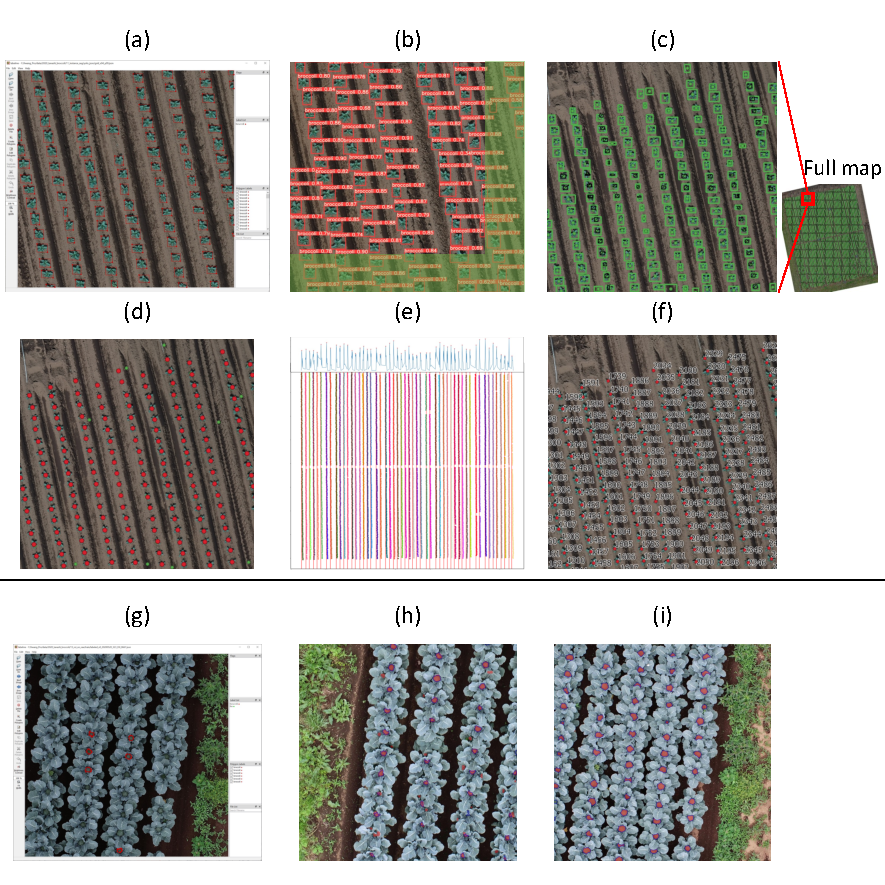
\includegraphics{figures/cp4/Fig.S1_deep_learning_demo.pdf}
    }
  \end{center}
  \caption[Examples of 2020 broccoli seedling position detection and head segmentation by interactive annotation]{
    Examples of 2020 broccoli seedling position detection (a-f) and head segmentation by interactive annotation (g-i). 
    (a) One annotated training data by LabelMe. 
    (b) YOLO v5 detected results; the green part is the buffer zone to avoid the broken broccoli at the edge. 
    (c) Duplicate detection in buffer zone removed by the non-maximum suppression (NMS) algorithm. Black shows removed duplicate detection, green shows those that were retained, and green dots are the center points as the broccoli position. 
    (d) Red dots show the manually adjusted positions by QGIS. 
    (e) Ridge detection by identifying the peak of points distribution. 
    (f) Automatic placing of plant ID along the ridge. 
    (g) Startup training data annotation made by LabelMe; only a few annotations were required. 
    (h) After the first iteration. The red polygons are the segmentation results (as auxiliary annotations) trained by the startup data and the blue polygons are manually adjusted according to the previous results. 
    (i) After the fourth iteration, almost no manual adjustment was required in this case.
  }
  \label{fig:cp4s1}
\end{figure}

\newpage

\begin{landscape}
  \begin{figure}[htb]
  \begin{center}
    \resizebox{\linewidth}{!}{
      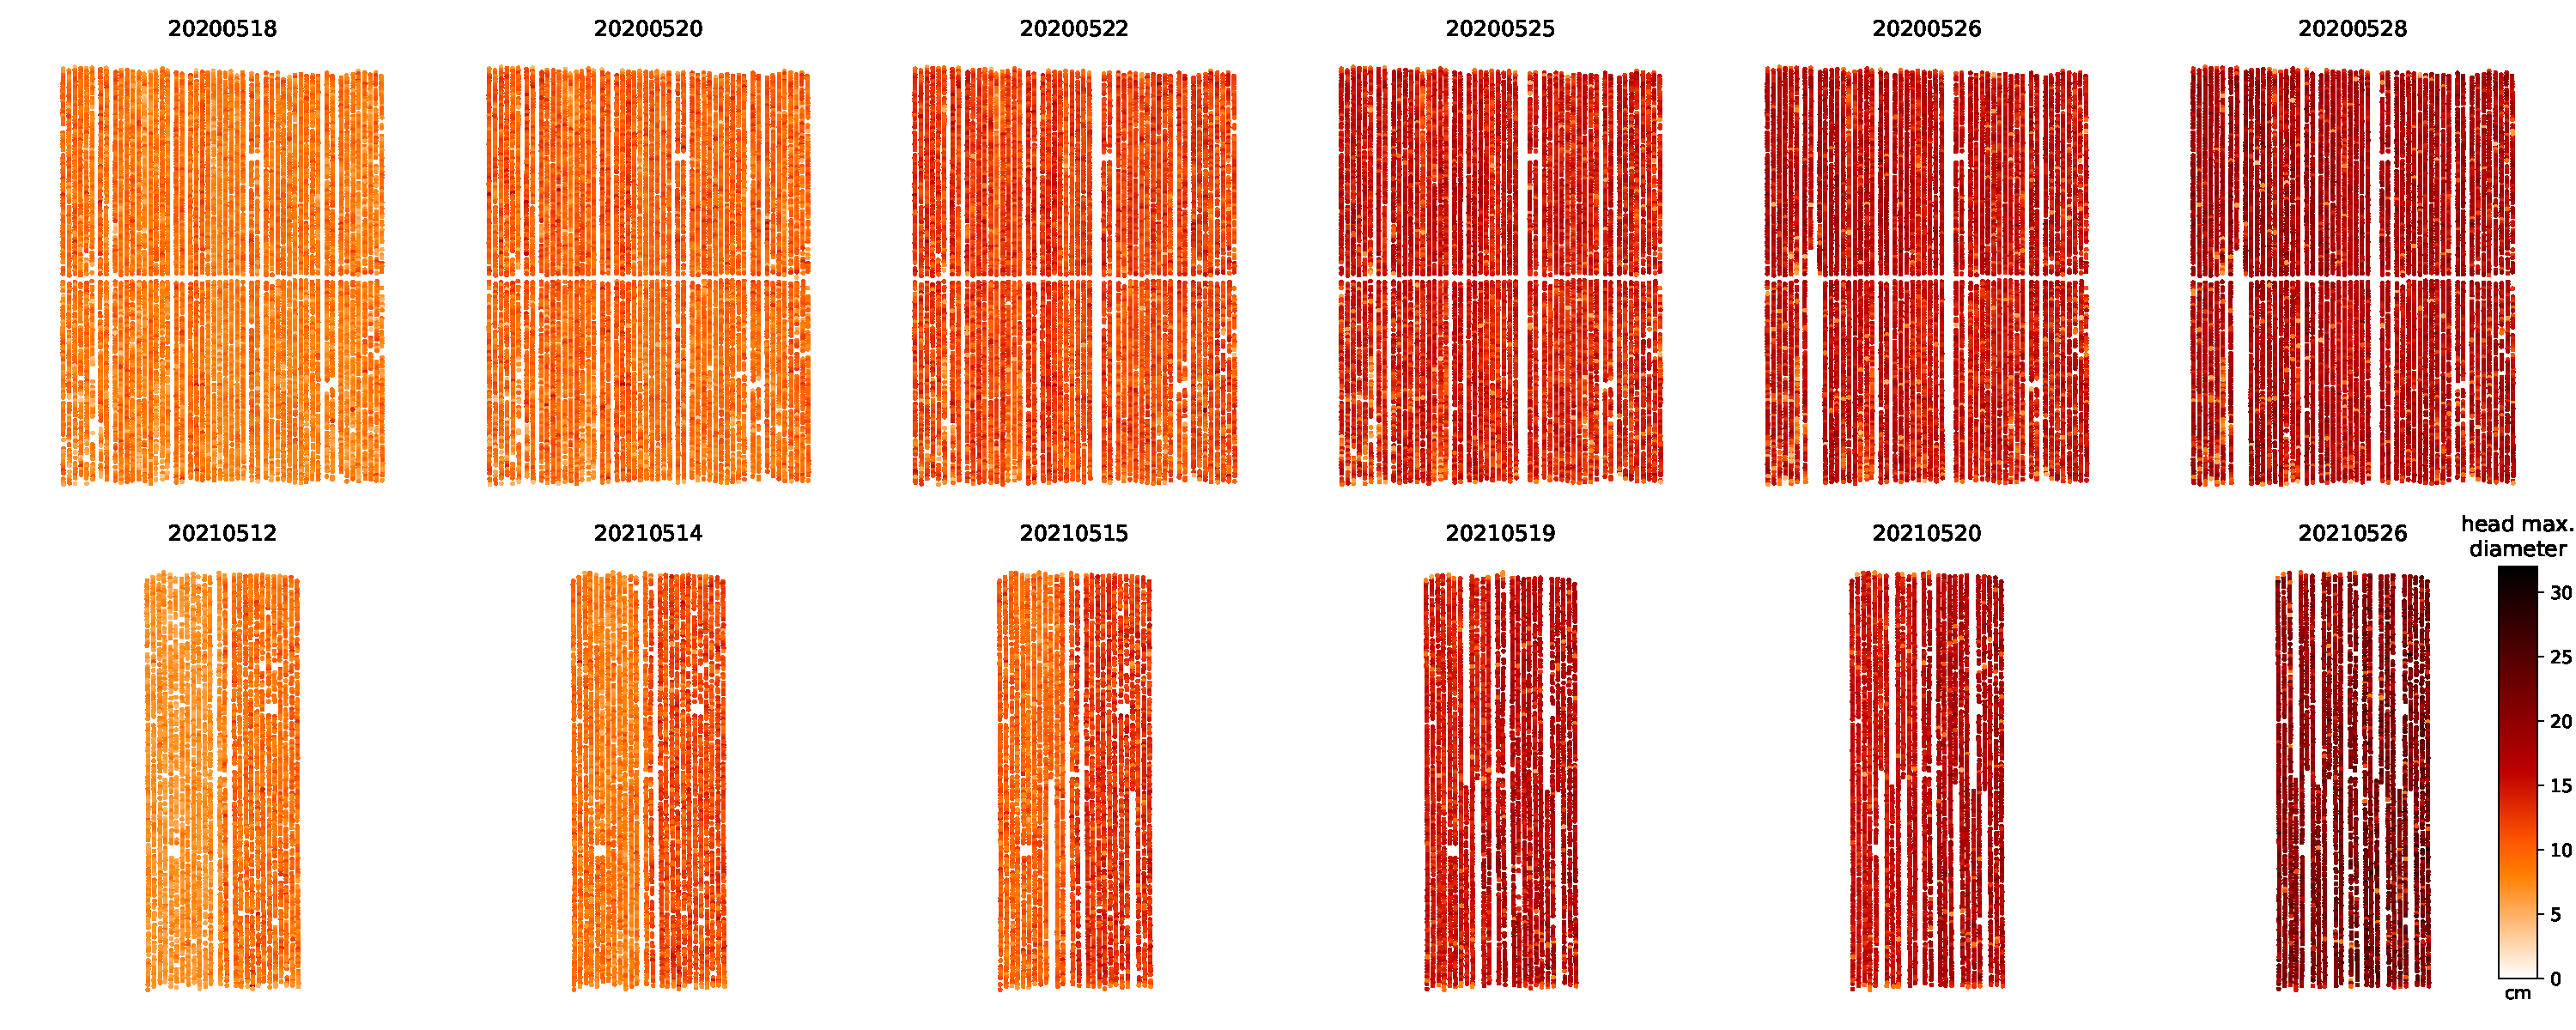
\includegraphics{figures/cp4/Fig.S2_plot_heatmap.pdf}
    }
  \end{center}
  \caption[Head size of all broccoli heads based on UAV imagery]{
    Head size of all broccoli heads based on UAV imagery; color represents the maximum head diameter.
  }
  \label{fig:cp4s2}
\end{figure}
\end{landscape}

\newpage

\begin{landscape}
  \begin{figure}[htb]
  \begin{center}
    \resizebox{0.9\linewidth}{!}{
      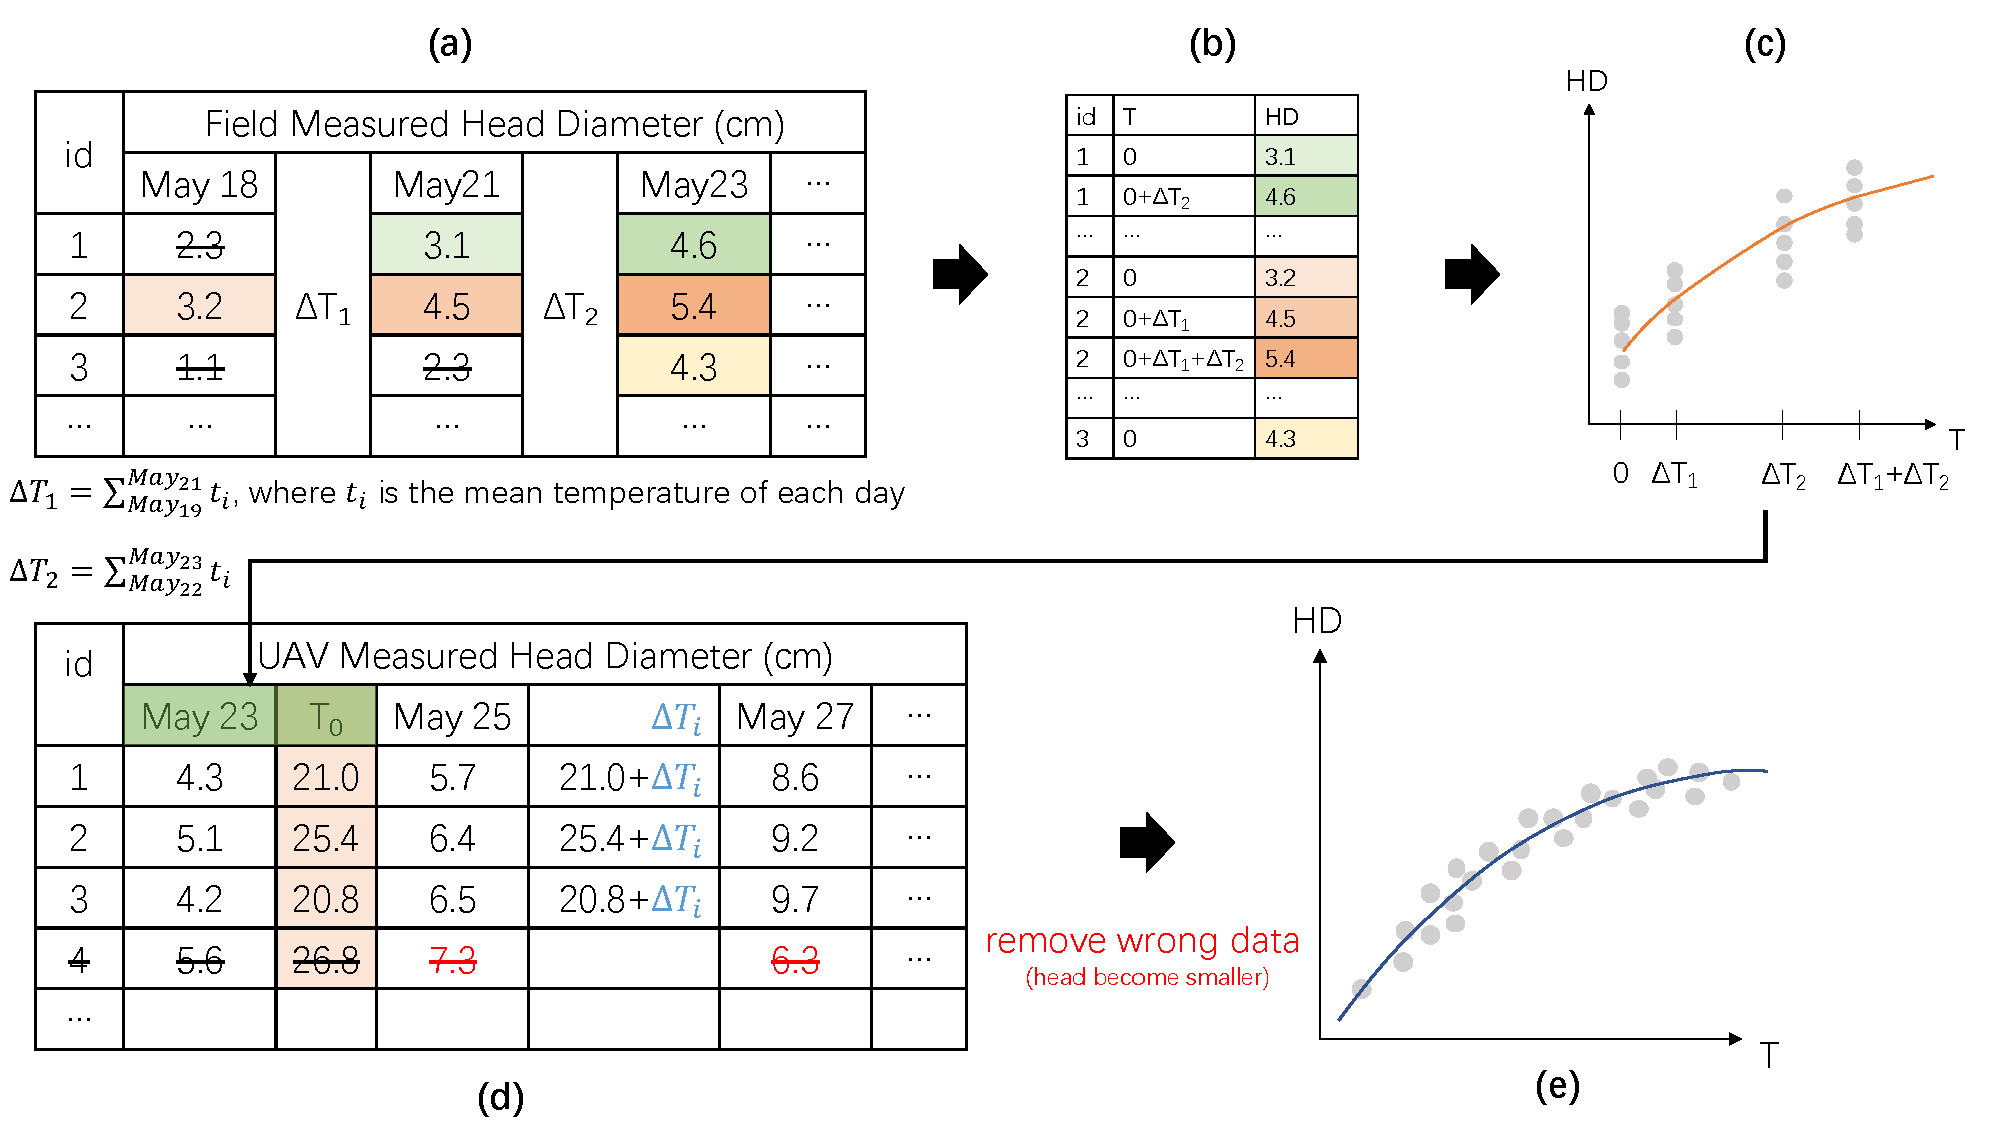
\includegraphics{figures/cp4/Fig.S3_yield_workflow.pdf}
    }
  \end{center}
  \caption[Data processing illustration for head size prediction model]{
    Data processing illustration for head size prediction model. All the numbers were just examples, not the actual results. 
    (a) The field-measured measured diameter at on different dates; the light colored was used as the starting date with broccoli head size around of approximately 3-3.5cm. $T$ is the sum of daily average temperature. $\Delta T_i$ is the temperature sum deviation. 
    (b) Reshaping of the previous table to a two-column table for the regression analysis shown in (c). 
    (d) The previous regressed model was used to initialize the $T$ from the head diameter. 
    $T$ on later days was added by the deviation $\Delta T_i$. 
    (e) the previous data was used to regress the prediction model from $T$ to head diameter.
  }
  \label{fig:cp4s3}
\end{figure}
\end{landscape}
